\section{Example: build low-dimensional models}\label{sec:nanostructure-examples}
\index{Nanoribbons}\index{Nanotubes}\index{Nanowires}

Cutting a sheet into a ribbon or rolling it into a tube changes its boundaries and periodicity. A ribbon has edges across its width and repeats only along its length. A nanotube repeats along its axis, with vacuum in the other directions. A wire cut from a bulk crystal likewise has one periodic direction, whereas a finite cluster is nonperiodic in all three.

This section first builds a 24-site graphene ribbon and a 32-site nanotube from a small primitive cell, then uses face-centered cubic copper to build a wire, finite cluster, and spherical void. Native JSON and CIF files accompany every result for comparison as you work.

\subsection{Prepare a 60-degree graphene primitive cell}

The supplied \file{nano-graphene-60.json} has two C sites, equal in-plane vector lengths of $2.46\,\text{\AA}$, an angle of $60^\circ$, and normal box height $15\,\text{\AA}$. It is periodic in-plane and nonperiodic along the normal. It represents the same graphene sheet as \file{graphene-layer.json}, using a different lattice basis.

Starting from the earlier $120^\circ$ cell, retain $\mathbf a$ and replace the second vector by $\mathbf a+\mathbf b$. The new vector still has length $2.46\,\text{\AA}$, but forms $60^\circ$ with $\mathbf a$. This integer basis change has determinant 1, so the model still has two independent sites. Both ribbon and tube examples use this $60^\circ$ input.

\begin{steps}
  \item Import \file{nano-graphene-60.json}, name it \file{nano-graphene}, and open its 3D document. Check for two independent sites, equal in-plane lengths, and $60^\circ$.
  \item To perform the basis change yourself, separately import and activate \file{graphene-layer.json}. Open \ui{Build Supercell} under \ui{Crystal Modeling}\,$\rightarrow$\,\ui{Supercell \& Lattice}.
  \item Enter \literalinput{1 0 0; 1 1 0; 0 0 1} under \ui{Supercell scaling}. This is a three-row integer matrix, with semicolons separating rows; it differs from editing individual cells in the lattice editor.
  \item Preview and check that the site count remains 2, volume is unchanged, and the in-plane angle becomes $60^\circ$. Apply and save under a basis-specific name without overwriting the $120^\circ$ monolayer.
  \item Retain separate inputs for the ribbon and nanotube. Start each construction from a monolayer; rolling an already cut ribbon would be a different procedure.
\end{steps}

The two cell boundaries look different, but describe the same periodic material. Check the input and basis before comparing site counts and dimensions. Widths or chiral indices alone do not fully specify the construction.

\subsection{Cut an armchair graphene nanoribbon}

Ribbon width and axial length are entered as repeat-unit counts; vacuum is in \AA. \ui{Armchair} and \ui{Zigzag} describe edge arrangements, not camera directions. Here choose armchair, inspect the paired carbon arrangement along the edges, then check connectivity along the periodic length.

\begin{table}[htbp]
\centering\small
\caption{Parameters for the 24-site armchair ribbon.}
\begin{tabularx}{\linewidth}{lX}
\toprule
Field & Input\\
\midrule
Width repetitions & 3, a dimensionless integer.\\
Axial repetitions & 2, a dimensionless integer.\\
Edge type & \ui{Armchair}.\\
Vacuum (Å) & 5; the tool adds this much on each side in both nonperiodic directions.\\
Maximum atom count & 500, an upper bound rather than a requested final count.\\
\bottomrule
\end{tabularx}
\end{table}

\begin{steps}
  \item Activate the prepared \file{nano-graphene} monolayer. Open \ui{Cut Nanoribbon} from \ui{Nanostructures} on \ui{Crystal Modeling}.
  \item Enter the table's values. Width 3 is not $3\,\text{\AA}$, and axial count 2 is not $2\,\text{\AA}$.
  \item Click \ui{Preview} and show the cell boundary. Inspect both edges along the sheet normal, then check from the side that the model is still flat.
  \item Check for 24 independent C sites. Inspect the periodic connections along the ribbon; the network near the two cell ends is not two disconnected molecules.
  \item Apply, name the result \file{graphene-armchair-w3-l2}, and save. Compare with the supplied JSON of the same name and retain the original monolayer separately.
\end{steps}

The result is periodic along global $y$, with native flags \literalinput{false true false}. Cell lengths are approximately $16.15$, $8.521690$, and $10.00\,\text{\AA}$. The axial period is $8.521690\,\text{\AA}$. The atoms span $6.15\,\text{\AA}$ across the width, plus $5\,\text{\AA}$ vacuum on each side, giving $16.15\,\text{\AA}$. The flat sheet has no normal thickness, so its normal box length is $10\,\text{\AA}$.

For the 24 unpassivated C atoms, a neighbor cutoff of $1.65\,\text{\AA}$ gives 16 atoms with three neighbors and 8 edge atoms with two. The shortest periodic distance is approximately $1.420282\,\text{\AA}$. This cutoff checks this carbon model; it is not a universal bonding distance. For hydrogen-passivated edges, save the unpassivated structure first, add hydrogen according to the intended edge coordination, and check composition.

\subsection{Roll graphene into a small nanotube}

First identify which in-plane vector becomes the circumference. The geometry described in the help is
\begin{equation}
  \mathbf C_h=n\mathbf a_1+m\mathbf a_2,
  \qquad R=\frac{\|\mathbf C_h\|}{2\pi}.
  \label{eq:nanotube-circumference-radius}
\end{equation}
Here $\mathbf a_1,\mathbf a_2$ are the input in-plane vectors in \AA; $n,m$ are dimensionless chiral indices; $\mathbf C_h$ is the chiral vector; and $R$ is the initial radius. The circumference is the magnitude of that vector combination. Vectors of equal length enclosing $60^\circ$ give $\|\mathbf C_h\|=a\sqrt{n^2+nm+m^2}$. For another basis, use Eq.~\eqref{eq:nanotube-circumference-radius} directly. This section retains the prepared $60^\circ$ basis: the same $(n,m)$ in different bases need not select the same rolling direction.

\begin{figure}[htbp]
\centering
\begin{tikzpicture}[x=1mm,y=1mm,font=\sffamily\small,>=stealth]
  \node[text=brand] at (26,54) {Rolling direction};
  \foreach \j in {0,1,2,3} {
    \draw[teal!55] ({6+4*\j},{10+7*\j}) -- ({38+4*\j},{10+7*\j});
    \foreach \i in {0,1,2,3,4} {
      \fill[brand] ({6+8*\i+4*\j},{10+7*\j}) circle (.8);
    }
  }
  \foreach \i in {0,1,2,3,4}
    \draw[teal!55] ({6+8*\i},10) -- ({18+8*\i},31);
  \draw[->,brand,line width=.9pt] (6,10) -- (38,10)
    node[midway,below=3pt] {$\mathbf C_h=4\mathbf a_1$};
  \draw[->,muted] (6,10) -- (14,10) node[above] {$\mathbf a_1$};
  \draw[->,muted] (6,10) -- (10,17) node[left] {$\mathbf a_2$};
  \draw[->,teal,line width=.8pt] (57,24) -- (69,24);
  \node[text=muted,font=\sffamily\footnotesize] at (63,32) {Join};
  \node[text=brand] at (95,54) {Fixed circumference};
  \fill[paleblue] (81,10) rectangle (109,39);
  \draw[brand,line width=.8pt] (81,10) -- (81,39);
  \draw[brand,line width=.8pt] (109,10) -- (109,39);
  \draw[brand,fill=paleblue,line width=.8pt] (95,39) ellipse (14 and 5);
  \draw[brand,line width=.8pt] (81,10) arc[start angle=180,end angle=360,x radius=14mm,y radius=5mm];
  \draw[brand,densely dashed] (109,10) arc[start angle=0,end angle=180,x radius=14mm,y radius=5mm];
  \draw[->,muted] (95,39) -- (109,39) node[midway,above] {$R$};
  \draw[->,teal] (115,10) -- (115,43) node[above] {Axis};
  \node[align=center,font=\sffamily\footnotesize] at (95,-1) {$\|\mathbf C_h\|=2\pi R$};
\end{tikzpicture}
\caption{Chiral vector and tube radius (schematic). The left panel shows lattice translation points and the $(4,0)$ direction that rolls into one circumference. The right panel relates the resulting circumference to its radius.}
\label{fig:nanotube-chiral-geometry}
\end{figure}


The chiral indices $(n,m)$ specify the circumferential lattice direction; axial repetitions set the number of translational periods along the tube. The small-radius $(4,0)$ example makes rolling, the seam, and periodicity easy to inspect. A relaxed equilibrium radius requires geometry optimization.

\begin{steps}
  \item Open a fresh monolayer from \file{nano-graphene-60.json} and activate it. Do not use the ribbon just created.
  \item Choose \ui{Roll Nanotube} under \ui{Nanostructures}. Enter 4 and 0 in the two \ui{Chiral indices (n m)} fields.
  \item Set \ui{Axial repetitions} to 2, \ui{Vacuum (Å)} to 6, and \ui{Maximum atom count} to 500.
  \item Preview the circular cross-section along the axis, then inspect the tube from the side. Rotate the camera to examine the seam and check periodic connections at the axial ends.
  \item Check for 32 C sites. Apply and save as \file{graphene-tube-4-0-l2}, retaining both monolayer and nanotube.
\end{steps}

The example is periodic along global $z$, with flags \literalinput{false false true}. Its rolling radius is
\[
 R=\frac{4\times2.46}{2\pi}\,\text{\AA}\approx1.566085\,\text{\AA}.
\]
Both transverse cell lengths are approximately $15.132169\,\text{\AA}$, the diameter plus $6\,\text{\AA}$ vacuum on each side. Axial length is approximately $8.521690\,\text{\AA}$. This transverse vacuum differs from total vacuum in the twisted-bilayer dialog; use each command's definition when checking box dimensions.

A periodic neighbor check on the saved coordinates finds three neighbors within $1.65\,\text{\AA}$ for every site, with a shortest distance of approximately $1.393202\,\text{\AA}$. Rolling a flat sheet onto a small circumference changes straight-line pair distances. Do not require every rolled C--C distance to remain exactly $1.420282\,\text{\AA}$. Check radius, seam, neighbors, and periodicity together, then relax the geometry separately.

\subsection{Inspect the tube end and side}

Import \file{graphene-tube-4-0-l2.json} directly to practice viewing before comparing other chiral indices. Initially retain \ui{Input cell} and \ui{1 × 1 × 1} so that the view represents one saved model period.

\begin{steps}
  \item Select the JSON through \ui{Home → Structure → Import structure from file...}. In Online, upload and then import it. Open the document and check for C and 32 sites.
  \item Click \ui{c} in the viewer toolbar, whose tooltip is \ui{View along c axis}. The tube axis is parallel to $c$, so this looks through its mouth. Inspect the carbon ring and central hollow region.
  \item Click \ui{a} or \ui{b} for a side view. Keep the same zoom and inspect the axial extent and curved hexagonal network. If spheres obscure bonds, reduce \ui{Atom scale} under \ui{Viewer settings → Style}.
  \item Show \ui{Unit cell} under \ui{Visibility} and compare the tube with its transverse vacuum box. Hide \ui{Boundary image atoms} to inspect one period's atoms, then show them again to check end connections.
  \item Under \ui{Scientific scene → Repeat cell}, change only \ui{c} to 2 and inspect the axial join. Use \ui{Reset to 1 × 1 × 1} afterward, then \ui{Reset camera} for an overall view.
  \item Export end and side views, recording that they show the same 32-site structure, with $(4,0)$ chirality, two axial repeats, and the original JSON filename.
\end{steps}

The hole in the axial view confirms a tubular arrangement. The side and repeated views help establish its axial periodicity. Display repetition does not create a larger calculation supercell, and extra boundary spheres are scene images; obtain the independent site count from the structure. Together, these views communicate diameter, length, and periodicity more clearly than one perspective view.

\begin{figure}[!htb]
\centering
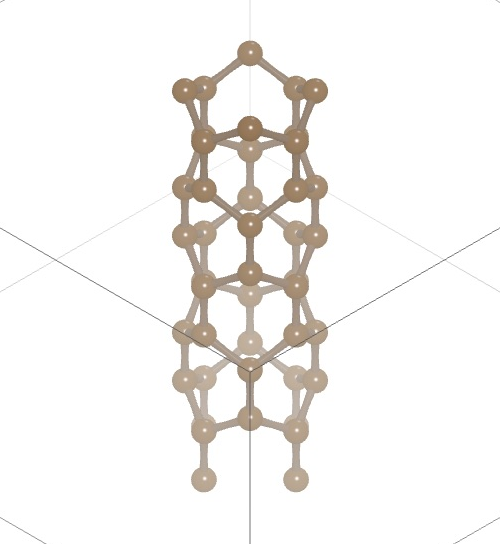
\includegraphics[width=.47\linewidth]{publication-assets/revision-nanotube-perspective.png}\hfill
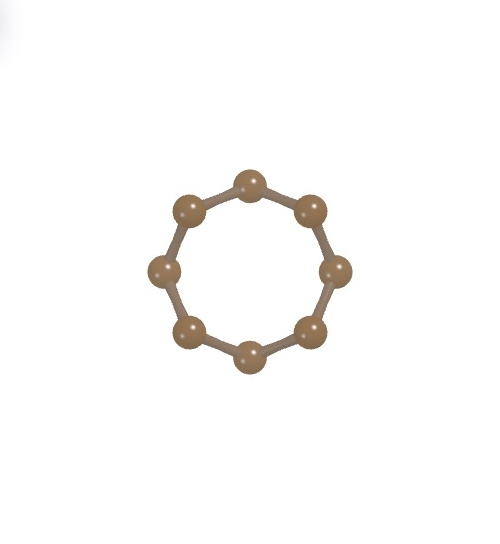
\includegraphics[width=.47\linewidth]{publication-assets/revision-nanotube-axis-c.png}
\caption{Two views of the same 32-site carbon nanotube. Left: inspect the curved network and axial connections from the side. Right: look down the tube into its hollow center. Periodic boundary images are displayed; the independent site count remains 32.}
\label{fig:nanotube-live}
\end{figure}

\FloatBarrier
\subsection{Cut a nanowire from copper}

Use \file{nano-Cu-fcc-input.json}, derived from the same four-site face-centered cubic cell as \file{Cu-fcc.cif}, with lattice constant $3.61\,\text{\AA}$. A nanowire retains translation along one lattice direction and selects a cross-section by radius. Atoms occupy discrete positions rather than forming a continuous medium: the outermost span of a spherical or cylindrical cut need not equal twice the entered radius.

Direction indices $[u\,v\,w]$ define the wire axis through the real-space lattice:
\begin{equation}
  \mathbf t=u\mathbf a+v\mathbf b+w\mathbf c.
  \label{eq:nanowire-lattice-direction}
\end{equation}
The dimensionless integers $u,v,w$ give $\mathbf t$ in the same length units as the lattice vectors. Construction uses an axis parallel to $\mathbf t$ and retains atoms within the specified transverse radius. Read the actual axial period from the output cell.

\begin{table}[htbp]
\centering
\caption{Direction indices and plane indices describe different geometry.}
\begin{tabularx}{\linewidth}{lX}
\toprule
Input & Geometry and use\\
\midrule
Direction $[u\,v\,w]$ & A combination of real-space $\mathbf a,\mathbf b,\mathbf c$, used for directions such as a wire axis.\\
Plane $(hkl)$ & A normal from reciprocal vectors, Eq.~\eqref{eq:surface-miller-normal}, used for surface cuts.\\
\bottomrule
\end{tabularx}
\end{table}

For cubic cells, a direction and the normal to a plane with the same indices are parallel; this is not generally true for oblique cells. Check whether the dialog asks for a direction or a plane, then inspect the preview axially and from the side.

\begin{steps}
  \item Import and activate the copper input, then open \ui{Cut Nanowire} under \ui{Nanostructures}.
  \item Enter 0, 0, 1 under \ui{Periodic direction (u v w)}. Set radius to $3\,\text{\AA}$, axial repetitions to 2, vacuum to $4\,\text{\AA}$, and maximum atom count to 2000.
  \item Inspect the preview cross-section along the axis and check that atoms lie within the selected cylinder. Check axial connections from the side and confirm 24 Cu sites.
  \item Apply and save as \file{Cu-wire-001-r3-l2}. Restart from bulk copper when changing radius or direction, rather than cutting an already finite cross-section as if it were bulk.
\end{steps}

The wire is periodic along $z$, with flags \literalinput{false false true} and axial cell length $7.22\,\text{\AA}$. Each transverse atomic span is $5.415\,\text{\AA}$. Adding $4\,\text{\AA}$ on each side gives transverse box lengths of $13.415\,\text{\AA}$. The shortest periodic neighbor distance is approximately $2.552655\,\text{\AA}$, matching bulk face-centered cubic Cu.

The atom limit also bounds the parent supercell needed for construction. This example uses 2000. If a smaller limit fails, inspect the required parent size in the message before adjusting it.

\begin{figure}[!htb]
\centering
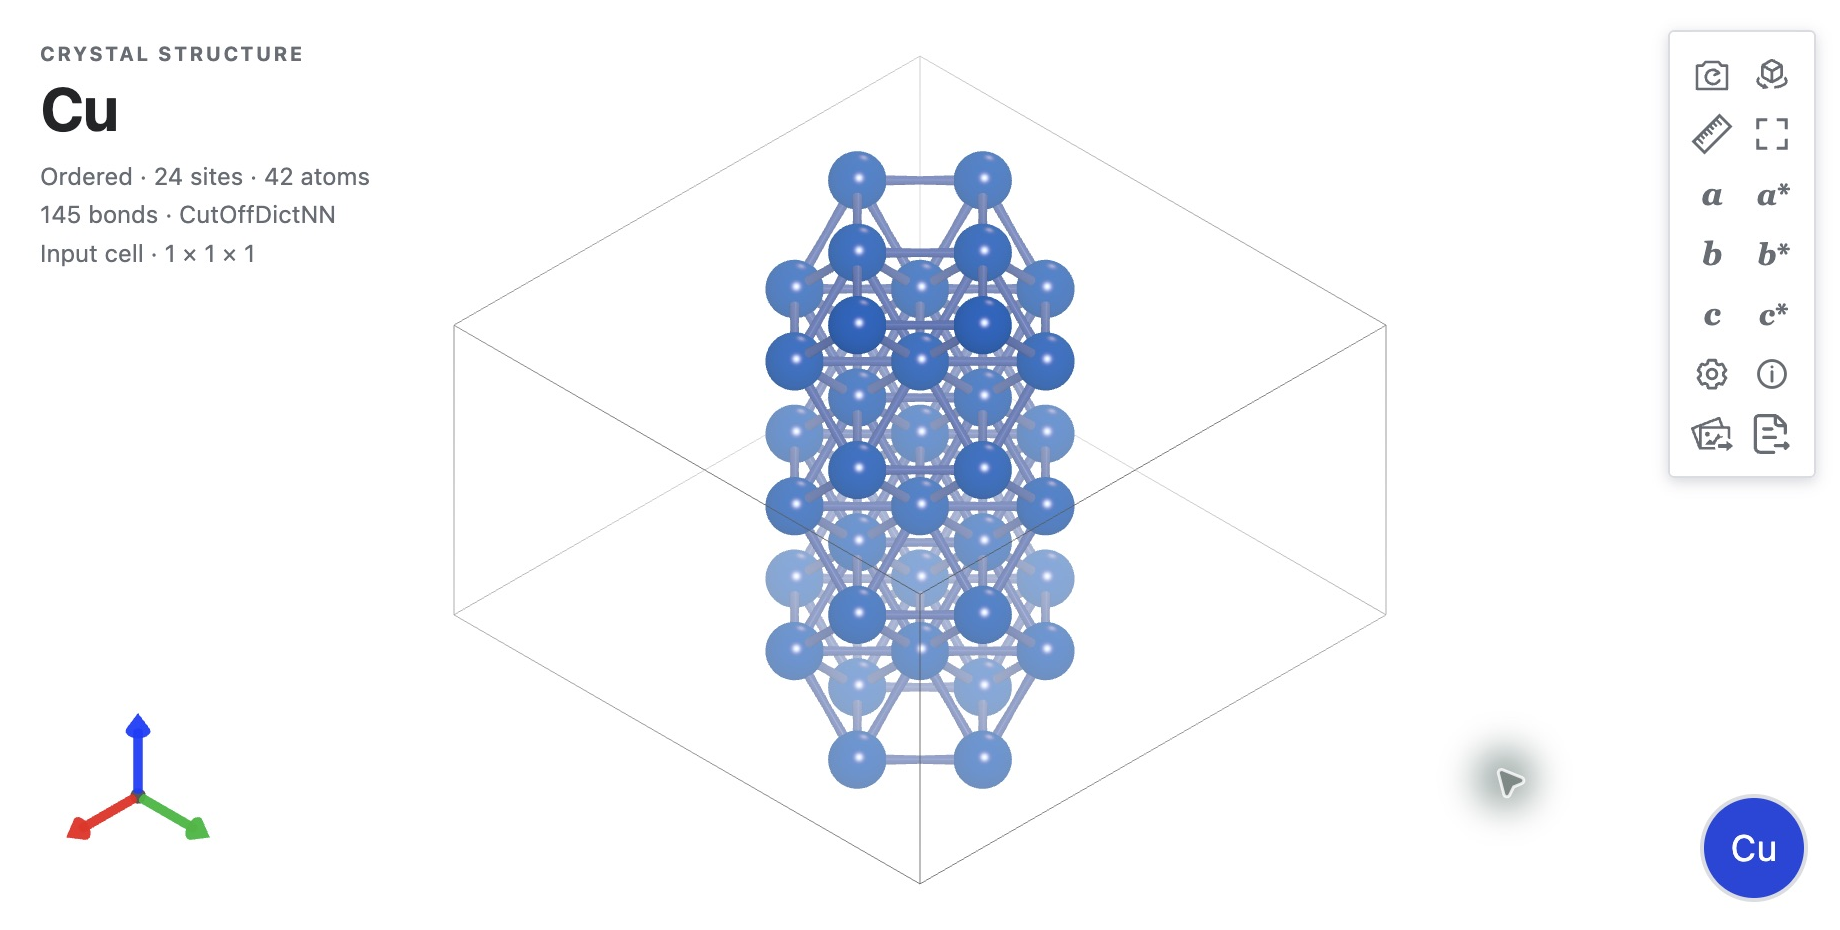
\includegraphics[width=\linewidth]{publication-assets/revision-nanowire-perspective.png}
\caption{The supplied 24-site copper nanowire in the viewer. Periodic boundary atoms show axial connectivity; transverse empty space is vacuum.}
\label{fig:nanowire-live}
\end{figure}

\FloatBarrier
\subsection{Inspect the wire's cross-section and axis}

Open \file{Cu-wire-001-r3-l2.json} to inspect the completed 24-site wire. Like the nanotube, it is periodic along $c$. The nanotube is made by rolling a sheet into a hollow cylinder; the copper wire retains crystal atoms inside a cylinder, including atoms within the cross-section.

\begin{steps}
  \item Import the JSON, open the document, and retain \ui{Input cell}. Check for Cu and 24 independent sites.
  \item Click \ui{c} to view down the axis. Discrete lattice positions may give a stepped outline rather than a smooth circle.
  \item Click \ui{a} or \ui{b} for a side view and show \ui{Unit cell}. The $7.22\,\text{\AA}$ axial length is the repeat period; the $13.415\,\text{\AA}$ transverse lengths accommodate the finite cross-section and vacuum.
  \item Clear unrelated selections and rotate slightly to show both end and side. Retain the cell boundary and orientation markers, and check that the view does not crop any atoms.
  \item If useful, set \ui{Repeat cell}'s \ui{c} to 2 to inspect connections, then restore one period. Save the project and structure. Record $[001]$, input radius $3\,\text{\AA}$, and 24 sites in exported figure captions.
\end{steps}

The input radius selects lattice positions; the retained discrete positions determine the actual outer span. The transverse span of $5.415\,\text{\AA}$ is smaller than diameter $6\,\text{\AA}$, consistent with the cut. Continue with suitable workflows for relaxation and electronic properties.

\subsection{Cut a finite copper cluster}
\index{Quantum dots}

The \ui{Quantum Dot} mode of \ui{Quantum Dot / Nano Void} retains atoms inside a sphere and makes the result nonperiodic in all three directions. This 13-site Cu cluster illustrates finite boundaries versus periodic bulk, and can be saved for subsequent electronic structure calculations.

\begin{steps}
  \item Reactivate the four-site copper input and open \ui{Quantum Dot / Nano Void} under \ui{Nanostructures}.
  \item Choose \ui{Quantum Dot}, radius $3\,\text{\AA}$, vacuum $4\,\text{\AA}$, and maximum atom count 2000.
  \item Preview and rotate the model. Check that no direction continues as an infinite atomic chain and that there are 13 Cu sites.
  \item Apply, name it \file{Cu-dot-r3}, and save the project and structure.
\end{steps}

All three cell lengths are approximately $11.61\,\text{\AA}$, while atoms span $3.61\,\text{\AA}$ in each direction. All periodicity flags are false. The shortest distance is approximately $2.552655\,\text{\AA}$. Using a $2.8\,\text{\AA}$ neighbor cutoff gives the central atom 12 neighbors and each of the 12 surface atoms 5. This initial cluster is cut directly from the face-centered cubic arrangement; its stable geometry requires optimization.

\subsection{Cut a spherical void in periodic copper}
\index{Nano voids}

Void mode retains the host outside the sphere and preserves the periodic box, the opposite of quantum-dot mode. Build a sufficiently large host first so that a small cell is not mostly or entirely removed.

\begin{steps}
  \item Import \file{Cu-void-host-2x2x2.json}, or use \ui{Build Supercell} on four-site Cu to make a $2\times2\times2$ host. Check for 32 Cu sites and cell lengths $7.22\,\text{\AA}$.
  \item Activate this host, open \ui{Quantum Dot / Nano Void}, choose \ui{Nano Void}, and set radius to $2.7\,\text{\AA}$. No external vacuum is needed around this periodic host.
  \item Preview with cell boundaries shown. The void center is fixed at host fractional position \((0.5,0.5,0.5)\). Check that central atoms are removed while the outer periodic host remains.
  \item Check that 13 atoms are removed, leaving 19 Cu sites. The cubic lattice remains $7.22\,\text{\AA}$ and periodic in all directions.
  \item Apply and save as \file{Cu-void-r2p7}, retaining the complete 32-site host for later radius changes or defect comparisons.
\end{steps}

The shortest periodic distance from the void center to a remaining atom is $3.61\,\text{\AA}$, larger than the input radius $2.7\,\text{\AA}$. This reflects discrete available lattice positions, not a failed radius setting. The host's shortest interatomic distance remains approximately $2.552655\,\text{\AA}$. Recording both the deletion-sphere radius and the closest remaining center-to-atom distance is clearer than a perspective view alone.

\subsection{Check periodicity and save the files}

Each native JSON retains its lattice, coordinates, periodicity flags, and construction metadata. CIF is used to exchange cell and atomic geometry, but these CIFs are imported as periodic in all directions. Use JSON to retain the low-dimensional periodicity in further modeling.

\begin{table}[htbp]
\centering\small
\caption{Site counts and native periodicity of the supplied nanostructures.}
\begin{tabularx}{\linewidth}{lX}
\toprule
Result & Model and key checks\\
\midrule
Graphene ribbon & 24C; periodic only in $y$; axial length $8.521690\,\text{\AA}$.\\
$(4,0)$ nanotube & 32C; periodic only in $z$; radius $1.566085\,\text{\AA}$.\\
Copper wire & 24Cu; periodic only in $z$; axial length $7.22\,\text{\AA}$.\\
Copper cluster & 13Cu; nonperiodic in all directions; cell lengths $11.61\,\text{\AA}$.\\
Copper with a void & 19Cu; periodic in all directions; 13 removed from a 32-site host.\\
\bottomrule
\end{tabularx}
\end{table}

\begin{steps}
  \item Save the project, giving inputs and derived results distinct names.
  \item For separate model files, choose JSON through \ui{Export file}\,$\rightarrow$\,\ui{Structure file}. Save CIF separately for geometry exchange. Do not choose the scene-oriented \ui{Scene JSON}.
  \item Reopen saved structures and check site count, cell, and periodic directions, then neighbors at edges, seams, or spherical cut boundaries.
  \item To regenerate these models, start MATLAB\regmark{} with \file{-nojvm}, configure the toolbox path, and run \file{nano_examples.m} from the examples directory. \file{verify_nano_examples.m} checks existing structures.
\end{steps}

These unpassivated starting models can be passivated, relaxed, and used in electronic structure calculations according to the material and boundaries. Retain both construction and calculation parameters, and confirm that the workflow references the intended structure.
